%!TEX program=xelatex

% 碰到Windows版本提示Fandol字体,可以在命令行中以管理员权限执行:tlmgr update -self -all
%\documentclass[review]{cvpr}
\documentclass[final]{cvpr}

\usepackage[UTF8]{ctex}

%\usepackage{cvpr}
\usepackage{times}
\usepackage{epsfig}
\usepackage{graphicx}
\usepackage{amsmath}
\usepackage{amssymb}
\usepackage{subfigure}
\usepackage{overpic}
% \usepackage{float}
\usepackage{stfloats}
\usepackage{enumitem}
\usepackage[noend]{algpseudocode}   %
\usepackage{setspace}   %
\setenumerate[1]{itemsep=0pt,partopsep=0pt,parsep=\parskip,topsep=5pt}
\setitemize[1]{itemsep=0pt,partopsep=0pt,parsep=\parskip,topsep=5pt}
\setdescription{itemsep=0pt,partopsep=0pt,parsep=\parskip,topsep=5pt}


\usepackage[pagebackref=true,breaklinks=true,colorlinks,bookmarks=false]{hyperref}


%\cvprfinalcopy % *** Uncomment this line for the final submission

\def\cvprPaperID{159} % *** Enter the CVPR Paper ID here
\def\confYear{CVPR 2020}
\def\httilde{\mbox{\tt\raisebox{-.5ex}{\symbol{126}}}}

\newcommand{\cmm}[1]{\textcolor[rgb]{0,0.6,0}{CMM: #1}}
\newcommand{\todo}[1]{{\textcolor{red}{\bf [#1]}}}
\newcommand{\alert}[1]{\textcolor[rgb]{.6,0,0}{#1}}

\newcommand{\IT}{IT\cite{98pami/Itti}}
\newcommand{\MZ}{MZ\cite{03ACMMM/Ma_Contrast-based}}
\newcommand{\GB}{GB\cite{conf/nips/HarelKP06}}
\newcommand{\SR}{SR\cite{07cvpr/hou_SpectralResidual}}
\newcommand{\FT}{FT\cite{09cvpr/Achanta_FTSaliency}}
\newcommand{\CA}{CA\cite{10cvpr/goferman_context}}
\newcommand{\LC}{LC\cite{06acmmm/ZhaiS_spatiotemporal}}
\newcommand{\AC}{AC\cite{08cvs/achanta_salient}}
\newcommand{\HC}{HC-maps }
\newcommand{\RC}{RC-maps }
\newcommand{\Lab}{$L^*a^*b^*$}
\newcommand{\mypara}[1]{\paragraph{#1.}}

\graphicspath{{figures/}}

% Pages are numbered in submission mode, and unnumbered in camera-ready
%\ifcvprfinal\pagestyle{empty}\fi
\setcounter{page}{1}


\renewcommand{\figref}[1]{图\ref{#1}}
\renewcommand{\tabref}[1]{表\ref{#1}}
\renewcommand{\equref}[1]{式\ref{#1}}
\renewcommand{\secref}[1]{第\ref{#1}节}
\def\abstract{\centerline{\large\bf 摘要} \hspace*{12pt} \it}

%%%%%%%%% TITLE 

\title{伪装物体检测}

\author{Deng-Ping Fan$^{1,2}$\quad Ge-Peng Ji$^{3}$ \quad Guolei Sun$^{4}$
    \quad Jianbing Shen$^{1,}$\thanks{通讯作者:Jianbing Shen (shenjianbingcg@gmail.com)}  \quad Ling Shao$^{1}$  \\
    $^{1}$ Inception Institute of Artificial Intelligence, UAE \quad$^{2}$College of CS, Nankai University, China\\
    \quad$^{3}$ School of Computer Science,Wuhan University, China \quad $^4$ETH Zurich, Switzerland 
}
\maketitle
\begin{document}

% \begin{center}
%     \centering
%     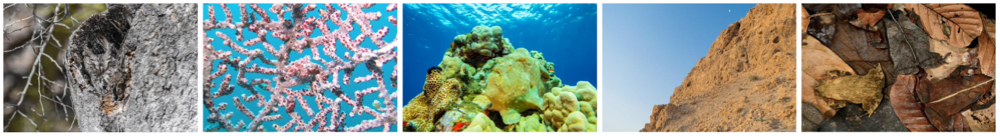
\includegraphics{COD_Zh_translate/figures/examples.png}
%     \label{fig:什么鸟屎}
% \end{center}




\begin{figure*}[tp]%这个好像成了
\centering
\subfigure
{
    \begin{minipage}[htbp]{.18\linewidth}
        \centering
        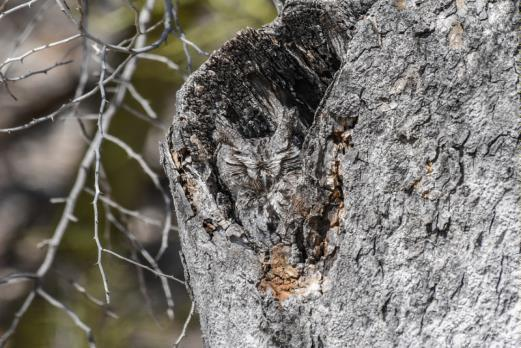
\includegraphics[scale=0.25]{COD_Zh_translate/figures/example1.png}
        \hspace{5mm} %调整纵向距离
    \end{minipage}
}
\subfigure
{
 	\begin{minipage}[htbp]{.18\linewidth}
        \centering
        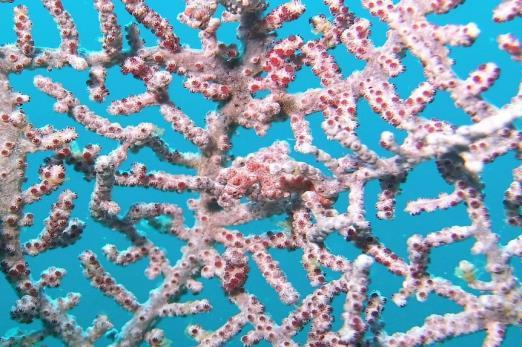
\includegraphics[scale=0.25]{COD_Zh_translate/figures/example2.png}
        \hspace{5mm} %调整纵向距离
    \end{minipage}
}
\subfigure
{
 	\begin{minipage}[htbp]{.18\linewidth}
        \centering
        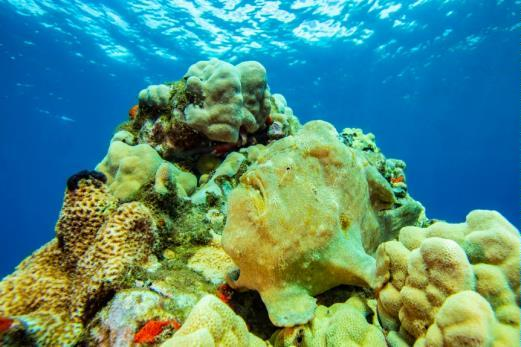
\includegraphics[scale=0.25]{COD_Zh_translate/figures/example3.png}
        \hspace{5mm} %调整纵向距离
    \end{minipage}
}
\subfigure
{
 	\begin{minipage}[htbp]{.18\linewidth}
        \centering
        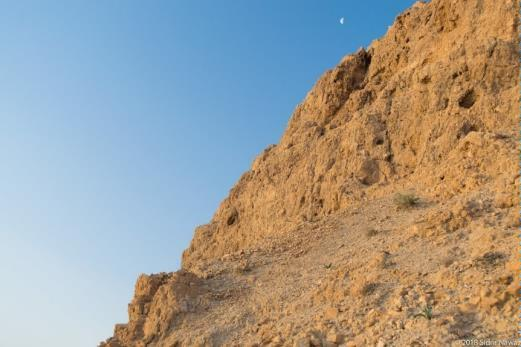
\includegraphics[scale=0.25]{COD_Zh_translate/figures/example4.png}
        \hspace{5mm} %调整纵向距离
    \end{minipage}
}
\subfigure
{
 	\begin{minipage}[htbp]{.18\linewidth}
        \centering
        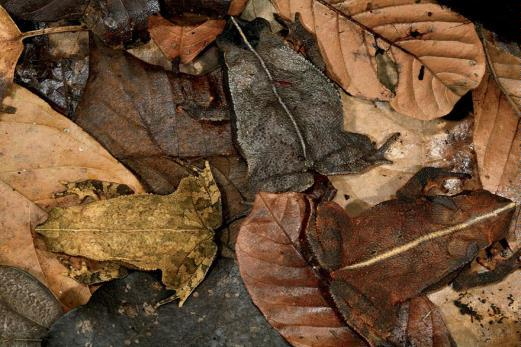
\includegraphics[scale=0.25]{COD_Zh_translate/figures/example5.png}
        \hspace{5mm} %调整纵向距离
    \end{minipage}
}
\caption{COD10K 数据集示例图。你能找到隐藏在图片中的伪装物体吗?以彩色电子版阅览时视觉效果最佳。 答案见补充材料。}
\label{fig:COD10K_examples}
\end{figure*}





%%%%%%%%% ABSTRACT
\begin{abstract}

\end{abstract}



%%%%%%%%% BODY TEXT %%%%%%%%%%%%%%%%%%%%%%%%%%%%%%%%%%%%%%%%
\section{引言}\label{sec:Introduction}

% \begin{figure}[h!]
%   \begin{overpic}[width=\columnwidth]{Comparison_COD.png} \small
%   \put(6,-4){(a)原图}
%   \put(26,-4){(b)通用物体}
%   \put(52,-4){(c)显著物体}
%   \put(76,-4){(d)伪装物体}
%     \end{overpic}\\
%     \caption{给定一张输入图像(a),(b)为全景分割 [31] 的真值(全景分割检测中的通用物体 [40,45]包括stuff和things),(c)是显著实例/物体检测 [17, 34, 62, 77](检测最吸引人注意力的目标),(d)是本文提出的伪装物体检测任务,即检测出与 周围环境具有相似模式(例如边缘,纹理或颜色)的物体。如 图所示,两只蝴蝶的边缘与香蕉融合在一起,难以识别。
%     }\label{fig:Comparsion_COD_SOD}
% \end{figure}





%%%%%%%%%%%%%%%%%%%%%%%%%%%%%%%%%%%%%%%%%%%%%%%%%%%%%%%%%%%%%%%%%%%%%%%%%%%%%%%%%
\section{相关工作}
\label{sec:RelatedWorks}



%%%%%%%%%%%%%%%%%%%%%%%%%%%%%%%%%%%%%%%%%%%%%%%%%%%%%%%%%%
\section{基于直方图统计的对比度}\label{sec:HC}

\section{基于区域的对比度}

%%%%%%%%%%%%%%%%%%%%%%%%%%%%%%%%%%%%%%%%%%%%%%%%%%%%%%%%%%%%%%%%%%%%%%
\section{实验比较}\label{sec:Experiment}



%%%%%%%%%%%%%%%%%%%%%%%%%%%%%%%%%%%%%%%%%%%%%%%%%

\section{总结与展望}\label{sec:Conclusion}



%引文我就只能意思一下了,COD原文引用太多了,我这边随便找齐了百多篇放到了bib里面,然后到时候我只能说随便引了,最后用goodnotes弄一下pdf

% {\small
% \bibliographystyle{ieee}
% \bibliography{COD_fake}
% }

% \end{CJK*}
\end{document}
